\documentclass[a6paper, parskip=half, DIV=14, 10pt]{scrartcl}
\usepackage{fontspec}
\usepackage[dvipsnames]{xcolor}
\usepackage{tikz}

\usepackage{booktabs}
\usepackage{multicol}
\setlength\columnsep{3em}
\usepackage{enumitem}
\usepackage{caption}
\usepackage{scrlayer-scrpage} % Manage headers and footers in Koma-Script document classes
\setlength{\footskip}{1cm}

\usepackage[type={CC}, version={4.0}, modifier={by}]{doclicense} % Add text and icons for creative commons license
\usepackage{array}
\usepackage{afterpage}

\usepackage[hidelinks]{hyperref} % Add hyperlinks to the pdf file. This should usually be the last package loaded before \begin{document}

\setmainfont{TeX Gyre Pagella}
\makeatletter
\newcommand{\version}[1]{\newcommand{\@version}{#1}}
\makeatother

% Set header
\clearpairofpagestyles
\makeatletter
\cfoot*{\normalshape Version \@version}
\makeatother

% Minimize unwanted hyphenation
\tolerance=1
\emergencystretch=\maxdimen
\hyphenpenalty=10000
\hbadness=10000

\setkomafont{section}{\setmainfont{Tex Gyre Pagella}\Large\bfseries}
\setkomafont{subsection}{\setmainfont{Tex Gyre Pagella}\large\bfseries}
\setkomafont{subsubsection}{\setmainfont{Tex Gyre Pagella}\normalsize\bfseries}
\setkomafont{descriptionlabel}{\setmainfont{Tex Gyre Pagella}\normalsize\bfseries}

\RedeclareSectionCommand[
  runin=false,
  afterindent=false,
  beforeskip=1cm,
  afterskip=0ex,
]{section}

\RedeclareSectionCommand[
  runin=false,
  afterindent=false,
  beforeskip=0pt,
  afterskip=0ex,
]{subsection}

\RedeclareSectionCommand[
  runin=false,
  afterindent=false,
  beforeskip=0pt,
  afterskip=0ex,
]{subsubsection}

\version{0.1}
\begin{document}
{%
\thispagestyle{empty}
		\enlargethispage{3.5\baselineskip} % Move the bottom line (author and date) down a bit
\setmainfont[Scale=1.0]{Tex Gyre Pagella}
\begin{center}
\makeatletter
{Version \@version}
\makeatother
\setmainfont[Scale=1.6]{Tex Gyre Pagella}

\Huge
Ceratopsians
\vfill{}
%\includegraphics[scale=0.375]{Images/triceratops_skull_cropped.png}
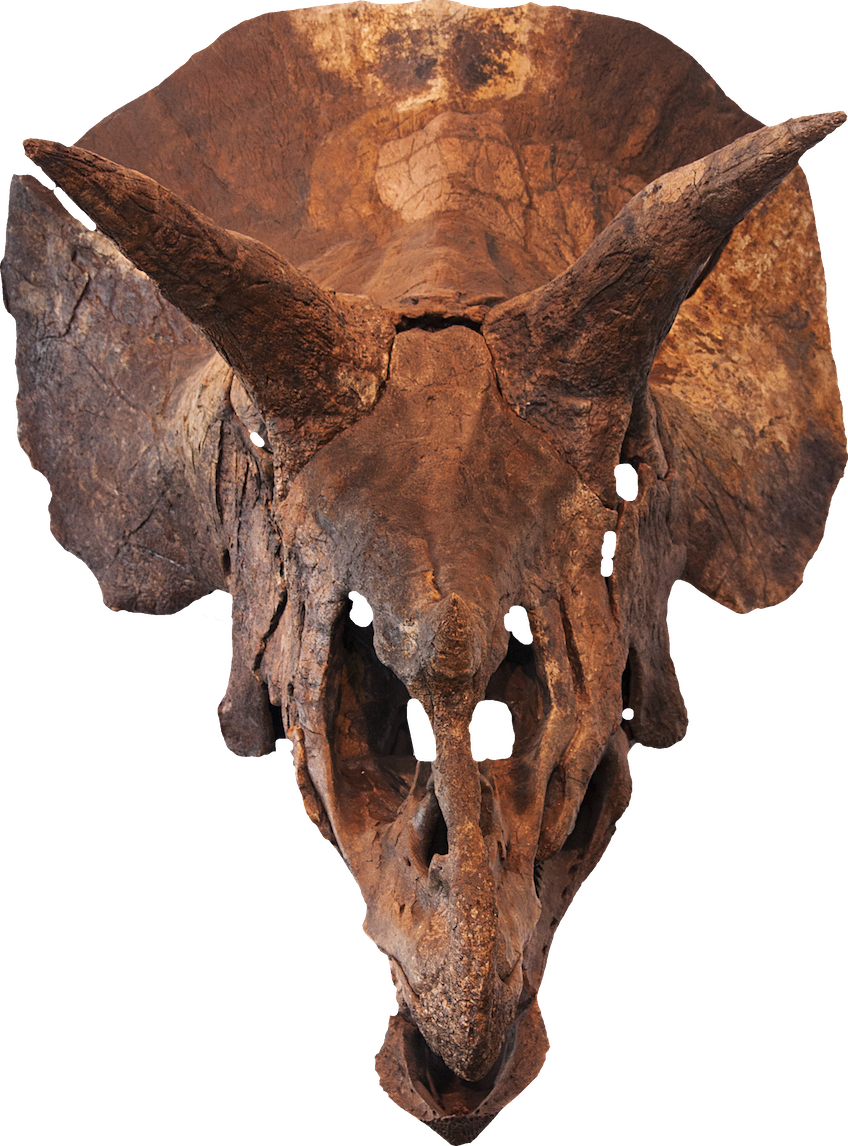
\includegraphics[scale=1.0]{Images/triceratops_skull_cropped2.png}
\vfill{}
\normalsize
Designed by Michael Purcell
\end{center}
}%
%\newpage
%\thispagestyle{empty}
%\phantom{a}

\newpage
\setmainfont{Tex Gyre Pagella}%
\raggedright%
\section*{Overview}
Ceratopsians is a card game for two players. It can be played in five to ten minutes and is intended for players who are at least eight years old.

During the game, you will assume the roles of rival paleontologists competing to see who can assemble the best displays of fossilized dinosaur skulls.


\section*{Components}
Ceratopsians is played with a set of eighteen cards. Unlike standard playing cards, these cards are two-sided. That is, they do not have a ``front'' side and a ``back'' side. Instead, each side represents one part of a fossilized dinosaur \emph{skull}.

There are six distinct skulls, each labeled with \emph{markers} in two colors: Red \& Yellow, Red \& Green, Red \& Blue, Yellow \& Green, Yellow \& Blue, and Green \& Blue.

The two sides of every card always represent parts of \emph{complementary} skulls. That is, they represent skulls that are labeled with disjoint sets of colors.

\newpage

Each skull is also divided into six parts: Left Frill, Center Frill, Right Frill, Left Cheek, Right Cheek, and~Mouth.

The two sides of every card always represent mirrored parts of their respective skulls.  That is, if one side represents a Left piece of a skull, the other represents the corresponding Right piece.  The Center Frill and the Mouth are their own mirrored parts. 

\textbf{Note}: There are only three Center Frill cards and three Mouth. The other skull parts (the Left and Right pieces) each appear on six cards.

\section*{Setup}
\begin{enumerate}[leftmargin=*]
	\item Shuffle the cards. Be sure to randomize both the order of the cards and their facings.
	\item Place the shuffled deck on the table within easy reach of all players.
	\item Place three cards on the table in a single column with one player seated at each end.
\end{enumerate}

\newpage

\section*{Playing the Game}
During the game, you will manipulate the cards in one of two possible ways: \emph{flipping} and \emph{sliding}. To flip a card, you will simply flip it over. To slide a card, you will move it from one place to another without flipping it.

The cards on the table comprise the \emph{boneyard}. Each card in the boneyard occupies one of three \emph{slots}.%is in one of three possible \emph{slots} in the boneyard.

On each of your turns you will \emph{draft} one card from the boneyard, thereby creating an \emph{empty} slot, and add it to your \emph{collection}. The cards in your collection will be used to create \emph{displays} at the end of the game.

On your turn you will:
\begin{enumerate}[leftmargin=*]
	\item \textbf{Draft a card from the boneyard.} Slide a card from any slot into your collection.
	\item \textbf{Update the boneyard.} Slide the card furthest from you into the slot furthest from you. Then, slide the other card into the middle slot. Flip any cards that you did not move.
	\item \textbf{Refill the boneyard.} Slide the top card of the deck into the slot closest to you.
\end{enumerate}
The game ends after both you and your opponent have drafted eight cards.

\newpage

\section*{Scoring}
After the game, you will assemble the cards in your collection into displays. Each display has six \emph{positions}, one corresponding to each of the skull parts. A \emph{complete} display is a display that has a card in all six positions.

Each card must be placed into the correct position within a display, but a display can contain parts from different skulls.
You may use the cards in your collection to create as many displays as you like.

You will score one point for every pair of colored markers that are aligned between adjacent cards in your displays. Only the colored markers that are filled in count for scoring purposes. You will score three bonus points for every complete display in your collection.

The player with the highest score wins the game.

%\newpage
%\section*{Example}

\vfill
\hrulefill

\textbf{Game Design}: Michael Purcell\\
\textbf{Contact}: \href{mailto:ceratopsians.game@gmail.com}{ceratopsians.game@gmail.com}\\
\begin{tabular}{@{}m{\columnwidth-\widthof{\Huge{\doclicenseIcon}}-0.5cm}@{\hspace{0.05cm}}m{\widthof{\Huge{\doclicenseIcon}}}@{}}
{\textbf{License}: This work is licensed\newline under a ``CC BY 4.0'' license.} & \Huge{\doclicenseIcon}\\
\end{tabular}

%\newpage
%\thispagestyle{empty}
%\phantom{a}
%
%\newpage
%\thispagestyle{empty}
%\phantom{a}
\end{document}
